\documentclass[12pt,a4paper]{report}

% Packages
\usepackage[utf8]{inputenc}
\usepackage{setspace}
\usepackage{geometry}
\usepackage{hyperref}
\usepackage{graphicx}

\usepackage{tikz}
\usetikzlibrary{arrows.meta, calc, positioning, patterns}

\tikzstyle{block} = [draw, fill=white, rectangle, 
    minimum height=3em, minimum width=6em]
\tikzstyle{sum} = [draw, fill=white, circle, node distance=1cm]
\tikzstyle{input} = [coordinate]
\tikzstyle{output} = [coordinate]
\tikzstyle{pinstyle} = [pin edge={to-,thin,black}]

\onehalfspacing
\geometry{margin=1in}

\begin{document}

\title{Reducing the runtime of an NP-Hard algorithm using deep learning on historical data}
\author{Christoffer Lindkvist}
\date{\today}
\maketitle

\begin{abstract}
    % SILKSONG SOON SHAW 
\end{abstract}

\tableofcontents
% \listoffigures

\chapter{Introduction}
\section{Background}
    This thesis is an extension to the Volvo Truck Assembly Line problem \cite{?}; 
    Today trucks are placed manually by management workers based solely on their own tacit knowledge, 
    thus none of those experience this is not written down anywhere. 
    The algorithm in the works will using data from Volvo help place the trucks so that there are as few overlaps as possible. 
    My idea is that the algorithm can gain a faster runtime by defaulting to "safe" combinations which are already used today.
    
\section{Research Problem}
The assemly line problem is considered NP-Hard, and the method today to solve this problem is based entirely on tacit knowledge. If this tacit knowledge could be emulated based on historical data we could get a better starting point and thus reduce the runtime needed for the heuristic algorithm. 
\section{Objectives}
The objectives of this thesis are:
\begin{enumerate}
    \item To design a deep learning model capable of emulating the tacit knowledge of Volvo's management workers using historical data.
    \item To integrate the model as a preprocessing step in the existing heuristic algorithm in order to reduce its runtime.
    \item To provide a visualization tool that intuitively illustrates the scheduling flow, highlighting overlaps and bottlenecks across stations and time.
\end{enumerate}
\section{Visualization of the Problem}
\subsection{UI/UX Problem}
    The UI will visualize the flow of the assembly line on two axes. One per station, and one in clockcycles. One clockcycle is the time it takes the theoretical items to make it from one station to the next. Hence the items must be displayed in a way that conveys that some stations take longer and shorter time to complete. In \autoref{fig:assembly} this is shown by stretching the items on the stations to better fit the clock cycles. One clockcycle is defined as a rudimentary unit of time, the size is arbitrary, and it does not reflect real life. For the sake of this thesis, we'll assume that one clockcycle is the time it takes for an arbitrary item $X$ to make it from $S_n$ to $S_{n+1}$ in one clockcycle, i.e. $T$ to $T + 1$.

    Issues in visualizing this way start to appearing when we start to consider that different stations $S_n$ and $S_m$ may take different times to complete. If we then step a clockcycle for each possible item, then we can never keep our items in sync. The main issue is that; if we compare the station $S_n$ and $S_m$, then we'll see that each station have a different time to finish, then the clockcycle system will not be perfect or even realistic as stations with differing times will each finish in different times and thus an item $X$ might make it to the station $S_{n+2}$
from $S_n$ in the same time it takes item $Y$ to make it to $S_{m+1}$ from $S_{m}$.


\begin{figure}[ht]
    \centering
    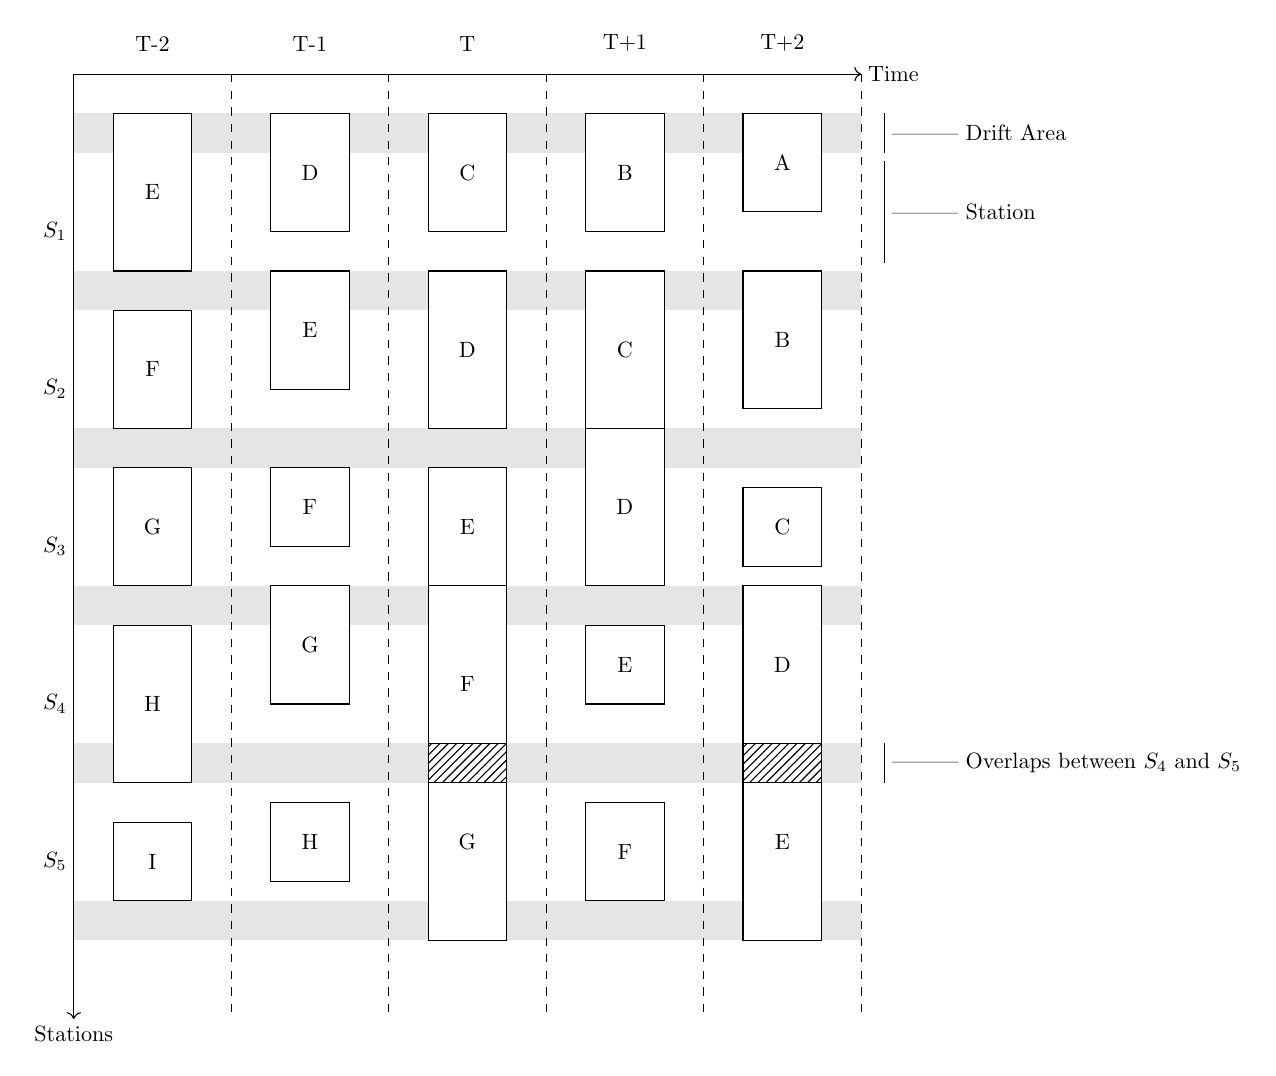
\begin{tikzpicture}[scale=1, every node/.style={scale=0.8, inner sep=3pt}]

        \foreach \y in {-1,-3,-5,-7,-9, -11} {
            \fill[gray!20] (0,\y+0.5) rectangle (10,\y);
        }

        \draw[->] (0,0) -- (10,0) node[right]{Time};
        \draw[->] (0,0) -- (0,-12) node[below]{Stations};

        \foreach \y/\name in { -2/$S_1$, -4/$S_2$, -6/$S_3$, -8/$S_4$, -10/$S_5$ } {
            \node[left] at (0,\y) { \name };
        }
        \draw[fill=white] (0.5,-9.5) rectangle (1.5,-10.5) node[midway]{I};

        \draw[fill=white] (0.5,-7) rectangle (1.5,-9) node[midway]{H};
        \draw[fill=white] (2.5,-9.25) rectangle (3.5,-10.25) node[midway]{H};

        \draw[fill=white] (0.5,-5) rectangle (1.5,-6.5) node[midway]{G};
        \draw[fill=white] (2.5,-6.5) rectangle (3.5,-8) node[midway]{G};
        \draw[fill=white] (4.5,-8.5) rectangle (5.5,-11) node[midway]{G};

        \draw[fill=white] (0.5,-3) rectangle (1.5,-4.5) node[midway]{F};
        \draw[fill=white] (2.5,-5) rectangle (3.5,-6) node[midway]{F};
        \draw[fill=white] (4.5,-6.5) rectangle (5.5,-9) node[midway]{F};
        \draw[fill=white] (6.5,-9.25) rectangle (7.5,-10.5) node[midway]{F};

        \draw[fill=white] (0.5,-0.5) rectangle (1.5,-2.5) node[midway]{E};
        \draw[fill=white] (2.5,-2.5) rectangle (3.5,-4) node[midway]{E};
        \draw[fill=white] (4.5,-5) rectangle (5.5,-6.5) node[midway]{E};
        \draw[fill=white] (6.5,-7) rectangle (7.5,-8) node[midway]{E};
        \draw[fill=white] (8.5,-8.5) rectangle (9.5,-11) node[midway]{E};

        \draw[fill=white] (2.5,-0.5) rectangle (3.5,-2) node[midway]{D};
        \draw[fill=white] (4.5,-2.5) rectangle (5.5,-4.5) node[midway]{D};
        \draw[fill=white] (6.5,-4.5) rectangle (7.5,-6.5) node[midway]{D};
        \draw[fill=white] (8.5,-6.5) rectangle (9.5,-8.5) node[midway]{D};

        \draw[fill=white] (4.5,-0.5) rectangle (5.5,-2) node[midway]{C};
        \draw[fill=white] (6.5,-2.5) rectangle (7.5,-4.5) node[midway]{C};
        \draw[fill=white] (8.5,-5.25) rectangle (9.5,-6.25) node[midway]{C};

        \draw[fill=white] (6.5,-0.5) rectangle (7.5,-2) node[midway]{B};
        \draw[fill=white] (8.5,-2.5) rectangle (9.5,-4.25) node[midway]{B};

        \draw[fill=white] (8.5,-0.5) rectangle (9.5,-1.75) node[midway]{A};

\draw[pattern=north east lines, pattern color=black] (4.5,-8.5) rectangle (5.5,-9) node[midway]{};
        
\draw[pattern=north east lines, pattern color=black] (8.5,-8.5) rectangle (9.5,-9) node[midway]{};


        % Vertical time slots with labels
        \foreach \x/\label in {2/T-2, 4/T-1, 6/T, 8/T+1, 10/T+2} {
            \draw[dashed] (\x,0) -- (\x,-12);
            \node[above] at (\x-1,0.2) {\label};
        }

        \draw (10.3,-0.5) -- (10.3,-1) node[midway,right]{|---| Drift Area };
        \draw (10.3,-1.1) -- (10.3,-2.4) node[midway,right]{|---| Station };

        \draw (10.3,-8.5) -- (10.3,-9) node[midway,right]{|---| Overlaps between $S_4$ and $S_5$};


    \end{tikzpicture}
    \caption{Assembly Line Example with Uniform Station and clockcycles}
    \label{fig:assembly}
\end{figure}

Thus we find the difficulty in displaying it properly in an intuitive graphical user interface. If we wish to display each station as uniform sizes, then we also have to stretch the items to make up for it visually. But doing this we have no intuitive way of knowing that $S_4$ could be 20 seconds long in real life, while $S_3$ could be 90. \textit{As luck would have it, each station at Volvo are each roughly 7 minutes long}, thus we will not run into any desync problems using clockcycles on these stations.

Between each station lies a buffer zone called a "drift area". A drift area in this case is the transitional area between any given station $S_n$ and $S_{n+1}$. Both of the stations can borrow time from each other within this area, but only one station may utilize that area at the time. This proves useful to help fit items that take longer on some stations onto the assembly line, but they are also the source of most problems.

As pictured in \autoref{fig:assembly}, $D$ will take a lot of time on $S_4$ and is forced to utilize time from $S_3$ and $S_5$. 
While this works well in a vacuum, the problems start to arise when $E$ also has to utilize additional time from its neighbouring stations, causing an overlap between $D$ and $E$ at $T+2$ as they both require the use of the drift area. 

The same problem arises with $F$ and $G$ at $T$ as both items need to borrow time from the stations before and after. Thus we run into another overlap.

Do note that on $T$, $E$ does not utilize the drift area which results in it sitting flush with $F$ on the timeline, this may look good on paper but can result in overlap in practice due to the human workers at the assembly line occasionally taking a bit longer than presumed. This can be resolved by borrowing some time from $S_2$ and moving $E$ into the drift area. 

The same issue arises at $T+1$ where $C$ and $D$ just barely get enough time, but it cannot get resolved by simply moving $D$ forward, as $D$ on $T+2$ will require all of the time it can get on $S_4$. 

\chapter{State of the art analysis}
\section{LSTM}

In previous works addressing similar scheduling problems, researchers have applied Recurrent Neural Networks (RNNs), often with Long Short-Term Memory (LSTM) units, in a sequence-to-sequence (seq2seq) framework. Seq2seq models are traditionally used in language-based tasks such as machine translation or text summarization, but the same architecture can be adapted to the assembly line problem.\cite{ref2} Each item can be represented as a vector, and a day’s worth of incoming items forms an input sequence of vectors. The seq2seq model can then be trained to output a corresponding placement sequence, effectively learning to replicate the tacit knowledge of the management workers in arranging the production items to minimize overlaps.\cite{ref3} 

The interesting part about LSTMs is that they can selectively forget irrelevant or outdated information through their forget gate. This helps them focus on more relevant patterns in the data over time, improving their ability to model long-term dependencies. \cite{ref4}

\section{Seq2Seq Models}
\section{Transformer-based Approaches}
\section{Heurestic Scheduling Methods}

\chapter{Methodology}
\section{The Heuristic Approach}

The problem to properly order manufacturing assembly lines with as few overlaps as possible is considered an NP-Hard problem. 

% \vspace{2em} 
\begin{figure}[ht]
    \centering

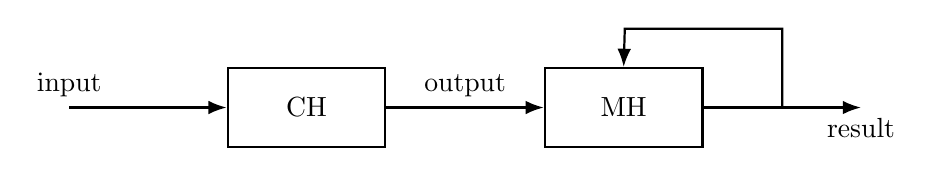
\begin{tikzpicture}[>=Latex, node distance=2cm, thick]

  \node[draw, minimum width=2cm, minimum height=1cm, align=center] (CH) {CH};
  \node[draw, minimum width=2cm, minimum height=1cm, align=center, right=of CH] (MH) {MH};

  \draw[->] ($(CH.west)+(-2,0)$) -- (CH.west) node[pos=0, above] {input};
  
  \draw[->] (CH.east) -- (MH.west) node[midway, above] {output};

  \draw[->] (MH.east) -- ++(1,0) -- ++(0,1) -- ++(-2,0) -- (MH.north);      

  \draw[->] (MH.east) -- ++(2,0) node[pos=1, below] {result};

\end{tikzpicture}
    \caption{Heuristic solution}
    \label{fig:solution}
\end{figure}

The Algorithm designed to solve this problem is a heuristic solution that will be made out of a Construction Hieuristic $(C\!H)$ that produces a starting point based on pre-defined constraints, that feeds into a Meta Heuristic $(M\!H)$ that finds a better solution starting from the output of the construction heuristic and self-improving until an acceptable result is returned. 

\section{Complementing the Heuristic Approach using Machine Learning}
Due to the fact that servicemen today place the items manually using tacit knowledge that they have accumulated over the years. Then what this thesis proposes is to emulate that same knowledge by learning which placement patterns tend to work together and which do not.

The idea is that if they have knowledge of an adequate solution from the get-go with some risk of overlap, then we can train a Deep Learning Model $(M\!L)$ on such previous data to give the algorithm a better starting point, thus (in theory) reducing the runtime of that algorithm.

\begin{figure}[ht]
    \centering
    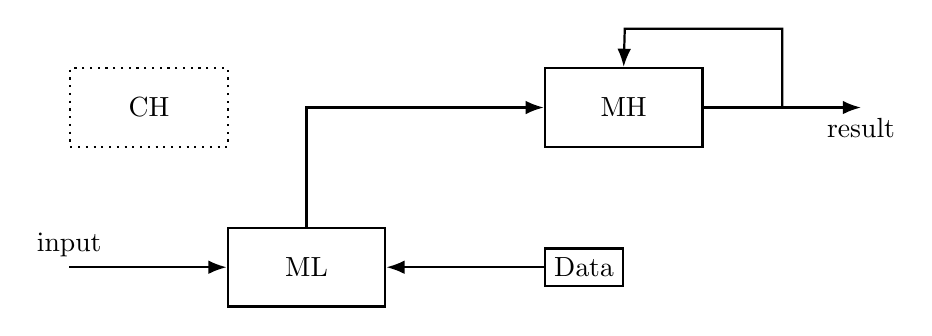
\begin{tikzpicture}[>=Latex, node distance=2cm, thick]
        \node[draw, minimum width=2cm, minimum height=1cm, align=center] (MH) {MH};
\node[draw, minimum width=2cm, minimum height=1cm, below left=1cm and 2cm of MH] (ML) {ML};
        \node[draw, align=center, right=of ML] (Data) {Data};
        \node[draw, dotted, minimum width=2cm, minimum height=1cm, align=center, left=4cm of MH] (CH) {CH};
        \draw[->] (MH.east) -- ++(1,0) -- ++(0,1) -- ++(-2,0) -- (MH.north);      

        \draw[->] (MH.east) -- ++(2,0) node[pos=1, below] {result};

        \draw[->] ($(ML.west)+(-2,0)$) -- (ML.west) node[pos=0, above] {input};

        \draw[->] (Data.west) -- (ML.east);

        \draw[->] (ML.north) |- (MH.west);

    \end{tikzpicture}
    \caption{ML solution}
    \label{fig:ml_solution}
\end{figure}

However it is worth to consider that such an approach can prove redundant or yield worse results if the problem at hand is an easy problem where many solutions can be found quickly, as opposed to a hard problem where a desired solution may not even be found. 

\section{System Architecture}

\chapter{Experiments and results}
\section{Dataset}
\section{Evaluation Metrics}
\section{Runtime Analysis}

\chapter{Discussion}
\section{Interpretation of Results}
\section{Limitations}
\section{Future Work}


\begin{thebibliography}{99}
\bibitem{ref1}
J. Abbasi, \textit{Predictive Maintenance in Industrial Machinery using Machine Learning}, 
Master’s thesis, Luleå University of Technology, Department of Computer Science, Electrical and Space Engineering, 2021.
\bibitem{ref2}
A. Dupuis, C. Dadouchi, and B. Agard, 
        \textit{A decision support system for sequencing production in the manufacturing industry},
\textit{Computers \& Industrial Engineering}, vol.~185, p.~109686, 2023. 
\bibitem{ref3} J. Lindén, 
    \textit{Understand and Utilise Unformatted Text Documents by Natural Language Processing Algorithms}, 
    Master’s thesis, Mid Sweden University, Department of Information and Communication Systems (IST), Spring 2017.
\bibitem{ref4} Ian Pointer,
\textit{Programming PyTorch for Deep Learning},
O'Reilly Media, 2019.
\bibitem{ref5} Author, Title, Journal, Year.
\bibitem{ref6} Author, Title, Journal, Year.
\bibitem{ref7} Author, Title, Journal, Year.
\bibitem{ref8} Author, Title, Journal, Year.
\bibitem{ref9} Author, Title, Journal, Year.
\bibitem{ref10} Author, Title, Journal, Year.
\bibitem{ref11} Author, Title, Journal, Year.
\bibitem{ref12} Author, Title, Journal, Year.
\bibitem{ref13} Author, Title, Journal, Year.
\bibitem{ref14} Author, Title, Journal, Year.
\bibitem{ref15} Author, Title, Journal, Year.
\bibitem{ref16} Author, Title, Journal, Year.
\bibitem{ref17} Author, Title, Journal, Year.
\bibitem{ref18} Author, Title, Journal, Year.
\bibitem{ref19} Author, Title, Journal, Year.
\bibitem{ref20} Author, Title, Journal, Year.
\end{thebibliography}
\end{document}
